\documentclass[]{article}
\usepackage{lmodern}
\usepackage{amssymb,amsmath}
\usepackage{ifxetex,ifluatex}
\usepackage{fixltx2e} % provides \textsubscript
\ifnum 0\ifxetex 1\fi\ifluatex 1\fi=0 % if pdftex
  \usepackage[T1]{fontenc}
  \usepackage[utf8]{inputenc}
\else % if luatex or xelatex
  \ifxetex
    \usepackage{mathspec}
  \else
    \usepackage{fontspec}
  \fi
  \defaultfontfeatures{Ligatures=TeX,Scale=MatchLowercase}
\fi
% use upquote if available, for straight quotes in verbatim environments
\IfFileExists{upquote.sty}{\usepackage{upquote}}{}
% use microtype if available
\IfFileExists{microtype.sty}{%
\usepackage{microtype}
\UseMicrotypeSet[protrusion]{basicmath} % disable protrusion for tt fonts
}{}
\usepackage[margin=1in]{geometry}
\usepackage{hyperref}
\hypersetup{unicode=true,
            pdftitle={662Midterm},
            pdfauthor={Ty Darnell},
            pdfborder={0 0 0},
            breaklinks=true}
\urlstyle{same}  % don't use monospace font for urls
\usepackage{color}
\usepackage{fancyvrb}
\newcommand{\VerbBar}{|}
\newcommand{\VERB}{\Verb[commandchars=\\\{\}]}
\DefineVerbatimEnvironment{Highlighting}{Verbatim}{commandchars=\\\{\}}
% Add ',fontsize=\small' for more characters per line
\usepackage{framed}
\definecolor{shadecolor}{RGB}{248,248,248}
\newenvironment{Shaded}{\begin{snugshade}}{\end{snugshade}}
\newcommand{\KeywordTok}[1]{\textcolor[rgb]{0.13,0.29,0.53}{\textbf{#1}}}
\newcommand{\DataTypeTok}[1]{\textcolor[rgb]{0.13,0.29,0.53}{#1}}
\newcommand{\DecValTok}[1]{\textcolor[rgb]{0.00,0.00,0.81}{#1}}
\newcommand{\BaseNTok}[1]{\textcolor[rgb]{0.00,0.00,0.81}{#1}}
\newcommand{\FloatTok}[1]{\textcolor[rgb]{0.00,0.00,0.81}{#1}}
\newcommand{\ConstantTok}[1]{\textcolor[rgb]{0.00,0.00,0.00}{#1}}
\newcommand{\CharTok}[1]{\textcolor[rgb]{0.31,0.60,0.02}{#1}}
\newcommand{\SpecialCharTok}[1]{\textcolor[rgb]{0.00,0.00,0.00}{#1}}
\newcommand{\StringTok}[1]{\textcolor[rgb]{0.31,0.60,0.02}{#1}}
\newcommand{\VerbatimStringTok}[1]{\textcolor[rgb]{0.31,0.60,0.02}{#1}}
\newcommand{\SpecialStringTok}[1]{\textcolor[rgb]{0.31,0.60,0.02}{#1}}
\newcommand{\ImportTok}[1]{#1}
\newcommand{\CommentTok}[1]{\textcolor[rgb]{0.56,0.35,0.01}{\textit{#1}}}
\newcommand{\DocumentationTok}[1]{\textcolor[rgb]{0.56,0.35,0.01}{\textbf{\textit{#1}}}}
\newcommand{\AnnotationTok}[1]{\textcolor[rgb]{0.56,0.35,0.01}{\textbf{\textit{#1}}}}
\newcommand{\CommentVarTok}[1]{\textcolor[rgb]{0.56,0.35,0.01}{\textbf{\textit{#1}}}}
\newcommand{\OtherTok}[1]{\textcolor[rgb]{0.56,0.35,0.01}{#1}}
\newcommand{\FunctionTok}[1]{\textcolor[rgb]{0.00,0.00,0.00}{#1}}
\newcommand{\VariableTok}[1]{\textcolor[rgb]{0.00,0.00,0.00}{#1}}
\newcommand{\ControlFlowTok}[1]{\textcolor[rgb]{0.13,0.29,0.53}{\textbf{#1}}}
\newcommand{\OperatorTok}[1]{\textcolor[rgb]{0.81,0.36,0.00}{\textbf{#1}}}
\newcommand{\BuiltInTok}[1]{#1}
\newcommand{\ExtensionTok}[1]{#1}
\newcommand{\PreprocessorTok}[1]{\textcolor[rgb]{0.56,0.35,0.01}{\textit{#1}}}
\newcommand{\AttributeTok}[1]{\textcolor[rgb]{0.77,0.63,0.00}{#1}}
\newcommand{\RegionMarkerTok}[1]{#1}
\newcommand{\InformationTok}[1]{\textcolor[rgb]{0.56,0.35,0.01}{\textbf{\textit{#1}}}}
\newcommand{\WarningTok}[1]{\textcolor[rgb]{0.56,0.35,0.01}{\textbf{\textit{#1}}}}
\newcommand{\AlertTok}[1]{\textcolor[rgb]{0.94,0.16,0.16}{#1}}
\newcommand{\ErrorTok}[1]{\textcolor[rgb]{0.64,0.00,0.00}{\textbf{#1}}}
\newcommand{\NormalTok}[1]{#1}
\usepackage{longtable,booktabs}
\usepackage{graphicx,grffile}
\makeatletter
\def\maxwidth{\ifdim\Gin@nat@width>\linewidth\linewidth\else\Gin@nat@width\fi}
\def\maxheight{\ifdim\Gin@nat@height>\textheight\textheight\else\Gin@nat@height\fi}
\makeatother
% Scale images if necessary, so that they will not overflow the page
% margins by default, and it is still possible to overwrite the defaults
% using explicit options in \includegraphics[width, height, ...]{}
\setkeys{Gin}{width=\maxwidth,height=\maxheight,keepaspectratio}
\IfFileExists{parskip.sty}{%
\usepackage{parskip}
}{% else
\setlength{\parindent}{0pt}
\setlength{\parskip}{6pt plus 2pt minus 1pt}
}
\setlength{\emergencystretch}{3em}  % prevent overfull lines
\providecommand{\tightlist}{%
  \setlength{\itemsep}{0pt}\setlength{\parskip}{0pt}}
\setcounter{secnumdepth}{0}
% Redefines (sub)paragraphs to behave more like sections
\ifx\paragraph\undefined\else
\let\oldparagraph\paragraph
\renewcommand{\paragraph}[1]{\oldparagraph{#1}\mbox{}}
\fi
\ifx\subparagraph\undefined\else
\let\oldsubparagraph\subparagraph
\renewcommand{\subparagraph}[1]{\oldsubparagraph{#1}\mbox{}}
\fi

%%% Use protect on footnotes to avoid problems with footnotes in titles
\let\rmarkdownfootnote\footnote%
\def\footnote{\protect\rmarkdownfootnote}

%%% Change title format to be more compact
\usepackage{titling}

% Create subtitle command for use in maketitle
\newcommand{\subtitle}[1]{
  \posttitle{
    \begin{center}\large#1\end{center}
    }
}

\setlength{\droptitle}{-2em}

  \title{662Midterm}
    \pretitle{\vspace{\droptitle}\centering\huge}
  \posttitle{\par}
    \author{Ty Darnell}
    \preauthor{\centering\large\emph}
  \postauthor{\par}
      \predate{\centering\large\emph}
  \postdate{\par}
    \date{October 24, 2018}


\begin{document}
\maketitle

\begin{enumerate}
\def\labelenumi{\arabic{enumi})}
\tightlist
\item
  I have not recieved any assistance from anyone in completing this
  exam.
\end{enumerate}

\section{Problem 2)}\label{problem-2}

\subsection{a)}\label{a}

\texttt{ga\_ultra} is the gestational age in weeks estimated by ultra
sound

\texttt{ga\_est} is the gestational age in weeks estimated at birth

A gestational age of 75 weeks is clearly impossible so I set this value
to missing in \texttt{ga\_ultra}.

\begin{Shaded}
\begin{Highlighting}[]
\NormalTok{ midt}\OperatorTok{$}\NormalTok{ga_ultra[midt}\OperatorTok{$}\NormalTok{ga_ultra}\OperatorTok{==}\DecValTok{75}\NormalTok{]=}\OtherTok{NA}
\KeywordTok{ggplot}\NormalTok{(}\DataTypeTok{data=}\NormalTok{midt,}\KeywordTok{aes}\NormalTok{(}\DataTypeTok{sample=}\NormalTok{ga_ultra))}\OperatorTok{+}\KeywordTok{geom_qq}\NormalTok{(}\DataTypeTok{na.rm =}\NormalTok{ T)}\OperatorTok{+}\KeywordTok{geom_qq_line}\NormalTok{(}\DataTypeTok{na.rm =}\NormalTok{ T)}
\end{Highlighting}
\end{Shaded}

\includegraphics{662midterm_files/figure-latex/unnamed-chunk-1-1.pdf}

Based on the qqplot, the \texttt{ga\_ultra} does not appear
approximately normally distributed.

\subsection{b)}\label{b}

\begin{Shaded}
\begin{Highlighting}[]
\NormalTok{mean.ultra=}\KeywordTok{mean}\NormalTok{(midt}\OperatorTok{$}\NormalTok{ga_ultra,}\DataTypeTok{na.rm=}\NormalTok{T)}
\NormalTok{mean.est=}\KeywordTok{mean}\NormalTok{(midt}\OperatorTok{$}\NormalTok{ga_est,}\DataTypeTok{na.rm=}\NormalTok{T)}
\NormalTok{ga_diff=midt}\OperatorTok{$}\NormalTok{ga_est}\OperatorTok{-}\NormalTok{midt}\OperatorTok{$}\NormalTok{ga_ultra}
\NormalTok{diff_mean=}\KeywordTok{mean}\NormalTok{(ga_diff,}\DataTypeTok{na.rm=}\NormalTok{T)}
\end{Highlighting}
\end{Shaded}

The mean of \texttt{ga\_ultra} is 38.7286534 and the mean of
\texttt{ga\_est} is 38.4122563.

The mean of the differences is -0.3180388

Although the data does not appear normally distributed, it is n large
enough (359 observations). In this scenario a t test is robust against
the assumption of normality.

\(\mu_{diff}\) = Mean of the differences between the two measures of
gestational age.

\(\alpha=.05\)

\(H_0= \mu_{diff}=0\)

\(H_A= \mu_{diff}\neq 0\)

\begin{Shaded}
\begin{Highlighting}[]
\NormalTok{(}\DataTypeTok{t=}\KeywordTok{t.test}\NormalTok{(ga_diff,}\DataTypeTok{alternative=}\StringTok{"two.sided"}\NormalTok{))}
\end{Highlighting}
\end{Shaded}

\begin{verbatim}
## 
##  One Sample t-test
## 
## data:  ga_diff
## t = -6.2677, df = 357, p-value = 1.057e-09
## alternative hypothesis: true mean is not equal to 0
## 95 percent confidence interval:
##  -0.4178305 -0.2182471
## sample estimates:
##  mean of x 
## -0.3180388
\end{verbatim}

\begin{Shaded}
\begin{Highlighting}[]
\NormalTok{pval=t}\OperatorTok{$}\NormalTok{p.value}
\end{Highlighting}
\end{Shaded}

Conclusion: Reject \(H_0\) since 1.0565891\times 10\^{}\{-9\}
\textless{} .05

There is evidence that the means of the two gestational age variables
differ.

\subsection{c)}\label{c}

We will use a Kolmogorov-Smirnoff test in order to detect if there is a
difference in the distributions of the two gestational age variables.

\(F_1\) = \texttt{ga\_ultra}

\(F_2\) = \texttt{ga\_est}

\(H_0:F_1(y)=F_2(y)\) for all y

\(H_A: F_1(y)\neq F_2(y)\) for at least one y

\(D=\max_y|F_{1n}(y)-F_{2m}(y)|\)

\(F_{1n}(y)\)= Emperical Distribution Function for the sample from
\(F_1\)

\(F_{2m}(y)\)= Emperical Distribution Function for the sample from
\(F_2\)

\begin{Shaded}
\begin{Highlighting}[]
\NormalTok{(}\DataTypeTok{k=}\KeywordTok{ks.test}\NormalTok{(midt}\OperatorTok{$}\NormalTok{ga_ultra,midt}\OperatorTok{$}\NormalTok{ga_est))}
\end{Highlighting}
\end{Shaded}

\begin{verbatim}
## 
##  Two-sample Kolmogorov-Smirnov test
## 
## data:  midt$ga_ultra and midt$ga_est
## D = 0.186, p-value = 8.216e-06
## alternative hypothesis: two-sided
\end{verbatim}

Using \(\alpha = .05\)

D=.186

p-value=8.2162289\times 10\^{}\{-6\}

since \(pvalue<.05\) reject \(H_0\)

We conclude that the distributions of \texttt{ga\_ultra} and
\texttt{ga\_est} may be different.

\subsection{d)}\label{d}

\begin{Shaded}
\begin{Highlighting}[]
\NormalTok{ga_estint=}\KeywordTok{cut}\NormalTok{(midt}\OperatorTok{$}\NormalTok{ga_est,}\KeywordTok{c}\NormalTok{(}\DecValTok{0}\NormalTok{,}\DecValTok{37}\NormalTok{,}\DecValTok{40}\NormalTok{,}\OtherTok{Inf}\NormalTok{),}\DataTypeTok{right=}\NormalTok{F,}\DataTypeTok{labels=}\KeywordTok{c}\NormalTok{(}\StringTok{"low"}\NormalTok{,}\StringTok{"med"}\NormalTok{,}\StringTok{"high"}\NormalTok{))}
\NormalTok{ga_ultraint=}\KeywordTok{cut}\NormalTok{(midt}\OperatorTok{$}\NormalTok{ga_ultra,}\KeywordTok{c}\NormalTok{(}\DecValTok{0}\NormalTok{,}\DecValTok{37}\NormalTok{,}\DecValTok{40}\NormalTok{,}\OtherTok{Inf}\NormalTok{),}\DataTypeTok{right=}\NormalTok{F,}\DataTypeTok{labels=}\KeywordTok{c}\NormalTok{(}\StringTok{"low"}\NormalTok{,}\StringTok{"med"}\NormalTok{,}\StringTok{"high"}\NormalTok{))}
\end{Highlighting}
\end{Shaded}

Breaking both versions of gestation age into intervals (low,med,high)
corresponding to (0,37), {[}37,40), {[}40,\(\infty\))

\begin{Shaded}
\begin{Highlighting}[]
\NormalTok{(}\DataTypeTok{k=}\KeywordTok{cohen.kappa}\NormalTok{(}\KeywordTok{cbind}\NormalTok{(ga_estint,ga_ultraint)))}
\end{Highlighting}
\end{Shaded}

\begin{verbatim}
## Call: cohen.kappa1(x = x, w = w, n.obs = n.obs, alpha = alpha, levels = levels)
## 
## Cohen Kappa and Weighted Kappa correlation coefficients and confidence boundaries 
##                  lower estimate upper
## unweighted kappa  0.61     0.68  0.75
## weighted kappa    0.77     0.77  0.77
## 
##  Number of subjects = 358
\end{verbatim}

Running a cohen kappa test in order to find the measure of agreement, we
get an unweighted kappa estimate of .68 with a 95\% CI (.61,.75). Since
kappa=0 if agreement is totally by chance and kappa=1 if there is
perfect agreement, a kappa of .68 indicates substantial agreement
according to the guidlines given Landis and Koch. Thus there is
substantial agreement between the two versions.

\subsection{e)}\label{e}

\begin{Shaded}
\begin{Highlighting}[]
\NormalTok{midt}\OperatorTok{$}\NormalTok{rand_month[midt}\OperatorTok{$}\NormalTok{rand_month}\OperatorTok\KeywordTok{c}\NormalTok{(}\DecValTok{0}\NormalTok{,}\DecValTok{15}\NormalTok{)]=}\OtherTok{NA}
\NormalTok{randomized=}\KeywordTok{table}\NormalTok{(midt}\OperatorTok{$}\NormalTok{rand_month)}
\NormalTok{days=}\KeywordTok{c}\NormalTok{(}\DecValTok{31}\NormalTok{,}\DecValTok{28}\NormalTok{,}\DecValTok{31}\NormalTok{,}\DecValTok{30}\NormalTok{,}\DecValTok{31}\NormalTok{,}\DecValTok{30}\NormalTok{,}\DecValTok{31}\NormalTok{,}\DecValTok{31}\NormalTok{,}\DecValTok{30}\NormalTok{,}\DecValTok{31}\NormalTok{,}\DecValTok{30}\NormalTok{,}\DecValTok{31}\NormalTok{)}
\NormalTok{rmonth=}\KeywordTok{rbind}\NormalTok{(randomized,days)}
\NormalTok{(}\DataTypeTok{cs=}\KeywordTok{chisq.test}\NormalTok{(rmonth))}
\end{Highlighting}
\end{Shaded}

\begin{verbatim}
## 
##  Pearson's Chi-squared test
## 
## data:  rmonth
## X-squared = 18.316, df = 11, p-value = 0.07454
\end{verbatim}

Since month values of 0 and 15 are invailed, I set those values to NA in
\texttt{rand\_month}. Assuming there are 28 days in February, ie not
leap year.

\(\pi_1 =\) women randomized each month

\(\pi_2 =\) days in each month

\(H_0 = \pi_1=\pi_2\)

\(H_A = \pi_1 \neq \pi_2\)

Conclusion: Fail to reject \(H_0\) since 0.0745401 \textgreater{} .05

There is not enough evidence to suggest that the number of women
randomized each month is not consistent with the number of days in each
month.

\subsection{f)}\label{f}

\begin{Shaded}
\begin{Highlighting}[]
\NormalTok{month2=}\KeywordTok{rbind}\NormalTok{(}\KeywordTok{table}\NormalTok{(midt}\OperatorTok{$}\NormalTok{rand_month),}\KeywordTok{table}\NormalTok{(midt}\OperatorTok{$}\NormalTok{birth_month))}
\KeywordTok{row.names}\NormalTok{(month2)=}\KeywordTok{c}\NormalTok{(}\StringTok{"rand_month"}\NormalTok{,}\StringTok{"birth_month"}\NormalTok{)}
\NormalTok{month2=}\KeywordTok{data.frame}\NormalTok{(}\KeywordTok{t}\NormalTok{(month2))}
\NormalTok{mon=}\DecValTok{1}\OperatorTok{:}\DecValTok{12}
\NormalTok{month2=}\KeywordTok{cbind}\NormalTok{(mon,month2)}
\end{Highlighting}
\end{Shaded}

\begin{Shaded}
\begin{Highlighting}[]
\NormalTok{f=}\KeywordTok{cbind}\NormalTok{(mon,month2}\OperatorTok{$}\NormalTok{rand_month,}\KeywordTok{rep}\NormalTok{(}\DecValTok{1}\NormalTok{,}\DataTypeTok{times=}\DecValTok{12}\NormalTok{))}
\NormalTok{g=}\KeywordTok{cbind}\NormalTok{(mon,month2}\OperatorTok{$}\NormalTok{birth_month,}\KeywordTok{rep}\NormalTok{(}\DecValTok{2}\NormalTok{,}\DataTypeTok{times=}\DecValTok{12}\NormalTok{))}
\NormalTok{h=}\KeywordTok{rbind}\NormalTok{(f,g)}
\KeywordTok{colnames}\NormalTok{(h)=}\KeywordTok{c}\NormalTok{(}\StringTok{"mon"}\NormalTok{,}\StringTok{"bothmonths"}\NormalTok{,}\StringTok{"i"}\NormalTok{)}
\NormalTok{h=}\KeywordTok{data.frame}\NormalTok{(h)}
\NormalTok{h}\OperatorTok{$}\NormalTok{i=}\KeywordTok{factor}\NormalTok{(h}\OperatorTok{$}\NormalTok{i)}
\KeywordTok{ggplot}\NormalTok{(}\DataTypeTok{data=}\NormalTok{h)}\OperatorTok{+}\KeywordTok{geom_boxplot}\NormalTok{(}\KeywordTok{aes}\NormalTok{(}\DataTypeTok{y=}\NormalTok{bothmonths,}\DataTypeTok{color=}\NormalTok{i))}
\end{Highlighting}
\end{Shaded}

\includegraphics{662midterm_files/figure-latex/unnamed-chunk-9-1.pdf}

Looking at the boxplots of the two variables, the number of women
randomized each month varies considerably more than the number of births
per month.

\subsection{g)}\label{g}

\begin{Shaded}
\begin{Highlighting}[]
\NormalTok{midt}\OperatorTok{$}\NormalTok{ppnum[midt}\OperatorTok{$}\NormalTok{ppnum}\OperatorTok{==-}\DecValTok{9}\NormalTok{]=}\OtherTok{NA}
\NormalTok{midt}\OperatorTok{$}\NormalTok{ppnum=}\KeywordTok{factor}\NormalTok{(midt}\OperatorTok{$}\NormalTok{ppnum,}\DataTypeTok{ordered=}\NormalTok{T)}
\NormalTok{preterm=}\KeywordTok{cut}\NormalTok{(midt}\OperatorTok{$}\NormalTok{ga_ultra,}\KeywordTok{c}\NormalTok{(}\DecValTok{0}\NormalTok{,}\DecValTok{37}\NormalTok{,}\OtherTok{Inf}\NormalTok{),}\DataTypeTok{right=}\NormalTok{F,}\DataTypeTok{labels=}\KeywordTok{c}\NormalTok{(}\DecValTok{1}\NormalTok{,}\DecValTok{0}\NormalTok{))}
\NormalTok{preterm=}\KeywordTok{fct_rev}\NormalTok{(}\KeywordTok{factor}\NormalTok{(preterm,}\DataTypeTok{ordered =}\NormalTok{ T))}
\NormalTok{tab2=}\KeywordTok{table}\NormalTok{(preterm,midt}\OperatorTok{$}\NormalTok{ppnum)}
\NormalTok{m=}\KeywordTok{apply}\NormalTok{(}\KeywordTok{matrix}\NormalTok{(tab2,}\DataTypeTok{nrow =} \DecValTok{2}\NormalTok{),}\DecValTok{2}\NormalTok{,rev)}
\NormalTok{tab3=}\KeywordTok{rbind}\NormalTok{(m,}\KeywordTok{colSums}\NormalTok{(m))}
\NormalTok{rnames=}\KeywordTok{c}\NormalTok{(}\StringTok{"preterm"}\NormalTok{,}\StringTok{"not preterm"}\NormalTok{,}\StringTok{"total"}\NormalTok{)}
\KeywordTok{rownames}\NormalTok{(tab3)=rnames}
 \KeywordTok{kable}\NormalTok{(tab3,}\DataTypeTok{caption =} \StringTok{"number of previous pregnancies"}\NormalTok{,}\DataTypeTok{col.names =} \KeywordTok{c}\NormalTok{(}\StringTok{"0"}\NormalTok{,}\StringTok{"1"}\NormalTok{,}\StringTok{"2"}\NormalTok{,}\StringTok{"3+"}\NormalTok{))}
\end{Highlighting}
\end{Shaded}

\begin{longtable}[]{@{}lrrrr@{}}
\caption{number of previous pregnancies}\tabularnewline
\toprule
& 0 & 1 & 2 & 3+\tabularnewline
\midrule
\endfirsthead
\toprule
& 0 & 1 & 2 & 3+\tabularnewline
\midrule
\endhead
preterm & 10 & 10 & 9 & 5\tabularnewline
not preterm & 57 & 117 & 72 & 28\tabularnewline
total & 67 & 127 & 81 & 33\tabularnewline
\bottomrule
\end{longtable}

We will need to use a Chi-Square test for trend in order to determine if
the risk of preterm delivery varies monotonically (increases or
decreases) with the number of of previous pregnancies.

\(\rho_1=\) P(preterm birth given 0 previous pregnancies)

\(\rho_2=\) P(preterm birth given 1 previous pregnancies)

\(\rho_3=\) P(preterm birth given 2 previous pregnancies)

\(\rho_4=\) P(preterm birth given 3+ previous pregnancies)

\(H_0: \rho_1=\rho_2=\rho_3=\rho_4\)

\(H_A: \rho_1 \rho_2 \rho_3 \rho_4\) increase or decrease monotonically

\(\mathcal{X}^2_{trend}\equiv \dfrac{[n_1x]^2}{[x^2]p(1-p)}\)

\begin{Shaded}
\begin{Highlighting}[]
\KeywordTok{prop.trend.test}\NormalTok{(}\KeywordTok{c}\NormalTok{(}\DecValTok{10}\NormalTok{,}\DecValTok{10}\NormalTok{,}\DecValTok{9}\NormalTok{,}\DecValTok{5}\NormalTok{),}\KeywordTok{c}\NormalTok{(}\DecValTok{67}\NormalTok{,}\DecValTok{128}\NormalTok{,}\DecValTok{81}\NormalTok{,}\DecValTok{33}\NormalTok{))}
\end{Highlighting}
\end{Shaded}

\begin{verbatim}
## 
##  Chi-squared Test for Trend in Proportions
## 
## data:  c(10, 10, 9, 5) out of c(67, 128, 81, 33) ,
##  using scores: 1 2 3 4
## X-squared = 0.0015348, df = 1, p-value = 0.9687
\end{verbatim}

Conclude the risk of preterm delivery does not vary monotonically with
the number of previous pregnancies.

\subsection{h)}\label{h}

\begin{Shaded}
\begin{Highlighting}[]
\NormalTok{tab4=}\KeywordTok{table}\NormalTok{(midt}\OperatorTok{$}\NormalTok{group,preterm)}
\NormalTok{prempred=}\KeywordTok{matrix}\NormalTok{(}\KeywordTok{c}\NormalTok{(}\DecValTok{149}\NormalTok{,}\DecValTok{23}\NormalTok{,}\DecValTok{172}\NormalTok{,}\DecValTok{171}\NormalTok{,}\DecValTok{16}\NormalTok{,}\DecValTok{187}\NormalTok{),}\DataTypeTok{byrow =}\NormalTok{ T,}\DataTypeTok{nrow =} \DecValTok{2}\NormalTok{)}
\NormalTok{(}\DataTypeTok{prempred=}\KeywordTok{rbind}\NormalTok{(prempred,}\KeywordTok{apply}\NormalTok{(prempred,}\DecValTok{2}\NormalTok{,sum)))}
\end{Highlighting}
\end{Shaded}

\begin{verbatim}
##      [,1] [,2] [,3]
## [1,]  149   23  172
## [2,]  171   16  187
## [3,]  320   39  359
\end{verbatim}

We will use Fisher's exact test in order to determine if treating
peridontal disease in pregnant women is effective in reducing the risk
of prematurity. We are looking to see if there is a statistically
significant difference between the proportion of women who have
nonpreterm deliveries between the prenatal peridonal treament group and
the control group (postpartum).

\(\pi_1\)= proportion of women with no preterm delivery in the treament
group.

\(\pi_2\)= proportion of women with no preterm delivery in the control
group.

\(H_0:\) P(no preterm\textbar{}treament)=P(no preterm\textbar{}control)

\(H_0: \pi_1=\pi_2\)

\(H_A:\) P(no preterm\textbar{}treament)\textgreater{}P(no
preterm\textbar{}control)

\(H_A: \pi_1>\pi_2\)

\begin{Shaded}
\begin{Highlighting}[]
\KeywordTok{fisher.test}\NormalTok{(}\KeywordTok{matrix}\NormalTok{(}\KeywordTok{c}\NormalTok{(}\DecValTok{149}\NormalTok{,}\DecValTok{23}\NormalTok{,}\DecValTok{171}\NormalTok{,}\DecValTok{16}\NormalTok{),}\DataTypeTok{nrow=}\DecValTok{2}\NormalTok{),}\DataTypeTok{alternative=}\StringTok{"greater"}\NormalTok{)}
\end{Highlighting}
\end{Shaded}

\begin{verbatim}
## 
##  Fisher's Exact Test for Count Data
## 
## data:  matrix(c(149, 23, 171, 16), nrow = 2)
## p-value = 0.9491
## alternative hypothesis: true odds ratio is greater than 1
## 95 percent confidence interval:
##  0.3227135       Inf
## sample estimates:
## odds ratio 
##  0.6070072
\end{verbatim}

Conclusion: Looking at the results of the Fisher Exact test, we see that
the pvalue is .9491\textgreater{}.05 so we fail to reject the null
hypothesis. Thus there is no evidence that the periodontal treatment is
effective in reducing prematurity.

\subsection{i)}\label{i}

\begin{Shaded}
\begin{Highlighting}[]
\NormalTok{pd_diff=midt}\OperatorTok{$}\NormalTok{pd_post}\OperatorTok{-}\NormalTok{midt}\OperatorTok{$}\NormalTok{pd_pre}
\end{Highlighting}
\end{Shaded}

\texttt{pd\_diff} is the difference in average pocket depth from
randomization to delievery. A negative value indicates a reduction in
pocket depth, thus less periodonal disease.

\(\mu_{diff}\)= mean of the differences of pocket depth

\(H_0:\) There is no difference between the means

\(H_0: \mu_{diff}=0\)

\(H_A:\) There is a difference between the means

\(H_A: \mu_{diff} \neq 0\)

\begin{Shaded}
\begin{Highlighting}[]
\KeywordTok{t.test}\NormalTok{(pd_diff,}\DataTypeTok{alternative=}\StringTok{"two.sided"}\NormalTok{)}
\end{Highlighting}
\end{Shaded}

\begin{verbatim}
## 
##  One Sample t-test
## 
## data:  pd_diff
## t = 3.0295, df = 285, p-value = 0.002674
## alternative hypothesis: true mean is not equal to 0
## 95 percent confidence interval:
##  0.02925257 0.13777288
## sample estimates:
##  mean of x 
## 0.08351273
\end{verbatim}

Conclusion: since p-value=.002674\textless{}.05

Reject \(H_0\), conclude there is a difference in the means of pocket
depth.

\subsection{j)}\label{j}

\begin{Shaded}
\begin{Highlighting}[]
\NormalTok{pd_}\DecValTok{1}\NormalTok{=midt}\OperatorTok\KeywordTok{filter}\NormalTok{(group}\OperatorTok{==}\DecValTok{1}\NormalTok{)}\OperatorTok\KeywordTok{transmute}\NormalTok{(}\DataTypeTok{pdchange1=}\NormalTok{pd_post}\OperatorTok{-}\NormalTok{pd_pre)}
\NormalTok{pd_}\DecValTok{2}\NormalTok{=midt}\OperatorTok\KeywordTok{filter}\NormalTok{(group}\OperatorTok{==}\DecValTok{2}\NormalTok{)}\OperatorTok\KeywordTok{transmute}\NormalTok{(}\DataTypeTok{pdchange2=}\NormalTok{pd_post}\OperatorTok{-}\NormalTok{pd_pre)}
\KeywordTok{ggplot}\NormalTok{(}\DataTypeTok{data=}\NormalTok{pd_}\DecValTok{1}\NormalTok{,}\KeywordTok{aes}\NormalTok{(}\DataTypeTok{sample=}\NormalTok{pdchange1))}\OperatorTok{+}\KeywordTok{geom_qq}\NormalTok{(}\DataTypeTok{na.rm =}\NormalTok{ T)}\OperatorTok{+}\KeywordTok{geom_qq_line}\NormalTok{(}\DataTypeTok{na.rm =}\NormalTok{ T)}
\end{Highlighting}
\end{Shaded}

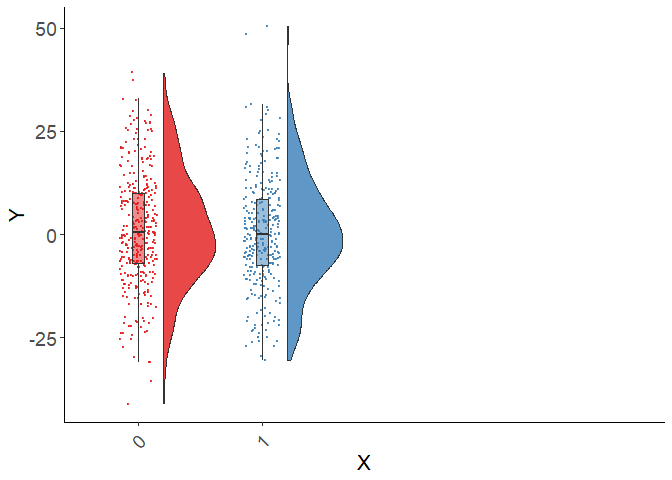
\includegraphics{662midterm_files/figure-latex/unnamed-chunk-16-1.pdf}

\begin{Shaded}
\begin{Highlighting}[]
\KeywordTok{ggplot}\NormalTok{(}\DataTypeTok{data=}\NormalTok{pd_}\DecValTok{2}\NormalTok{,}\KeywordTok{aes}\NormalTok{(}\DataTypeTok{sample=}\NormalTok{pdchange2))}\OperatorTok{+}\KeywordTok{geom_qq}\NormalTok{(}\DataTypeTok{na.rm =}\NormalTok{ T)}\OperatorTok{+}\KeywordTok{geom_qq_line}\NormalTok{(}\DataTypeTok{na.rm =}\NormalTok{ T)}
\end{Highlighting}
\end{Shaded}

\includegraphics{662midterm_files/figure-latex/unnamed-chunk-16-2.pdf}

\begin{Shaded}
\begin{Highlighting}[]
\NormalTok{pd1_m=}\KeywordTok{mean}\NormalTok{(pd_}\DecValTok{1}\OperatorTok{$}\NormalTok{pdchange1,}\DataTypeTok{na.rm=}\NormalTok{T)}
\NormalTok{pd2_m=}\KeywordTok{mean}\NormalTok{(pd_}\DecValTok{2}\OperatorTok{$}\NormalTok{pdchange2,}\DataTypeTok{na.rm=}\NormalTok{T)}
\end{Highlighting}
\end{Shaded}

Looking at the qqplots of the two groups, the data appears approximately
normally distributed. In addition we have a large sample size so the
data is n large enough. Based on this I have selected a two sample ttest
in order to determine if the mean change in pre and post pocket depth
differs between the two groups. Not assuming that the variance is equal
between the two groups.

\(pd_1\) = change in pocket depth for treatment group, negative values
indication reduction in pocket depth, thus less periodontal disease.
Mean for this group is \(\mu_1=\)-0.0129534

\(pd_2\) = change in pocket depth for control group, negative values
indication reduction in pocket depth, thus less periodontal disease.
Mean for this group is \(\mu_2\) = 0.166198

\(H_0: \mu_1=\mu_2\) (No change)

\(H_A: \mu_1 \neq \mu_2\) (The mean change differs between the two
groups)

\begin{Shaded}
\begin{Highlighting}[]
\KeywordTok{t.test}\NormalTok{(pd_}\DecValTok{1}\NormalTok{,pd_}\DecValTok{2}\NormalTok{,}\DataTypeTok{var.equal =}\NormalTok{ F)}
\end{Highlighting}
\end{Shaded}

\begin{verbatim}
## 
##  Welch Two Sample t-test
## 
## data:  pd_1 and pd_2
## t = -3.261, df = 262.16, p-value = 0.001257
## alternative hypothesis: true difference in means is not equal to 0
## 95 percent confidence interval:
##  -0.28732485 -0.07097795
## sample estimates:
##   mean of x   mean of y 
## -0.01295341  0.16619799
\end{verbatim}

Looking at the p-value, .001257\textless{}.05 so reject \(H_0\)

Conclude there is a difference between the mean change in average pocket
depth between the two groups.

\subsection{k)}\label{k}

While there was a reduction in pocket depth in the treament group from
randomization to delivery, thus a reduction in periodontal disease, it
does not seem that this had an effect on birthweight since there was not
a statistically significant difference in birth weights between the
treatment and control group. One possible explanation is that
periodontal disease during pregnancy is not a factor for birthweight.

\section{Problem 3)}\label{problem-3}

\subsection{a)}\label{a-1}

\begin{Shaded}
\begin{Highlighting}[]
\NormalTok{pdtab1=}\KeywordTok{table}\NormalTok{(cc}\OperatorTok{$}\NormalTok{ei_pd,cc}\OperatorTok{$}\NormalTok{ci_pb)}
\NormalTok{pdtab=}\KeywordTok{matrix}\NormalTok{(}\KeywordTok{c}\NormalTok{(}\DecValTok{36}\NormalTok{,}\DecValTok{18}\NormalTok{,}\DecValTok{54}\NormalTok{,}\DecValTok{51}\NormalTok{,}\DecValTok{69}\NormalTok{,}\DecValTok{120}\NormalTok{,}\DecValTok{87}\NormalTok{,}\DecValTok{87}\NormalTok{,}\DecValTok{174}\NormalTok{),}\DataTypeTok{nrow=}\DecValTok{3}\NormalTok{,}\DataTypeTok{byrow=}\NormalTok{T)}
\NormalTok{pdtab1=}\KeywordTok{matrix}\NormalTok{(}\KeywordTok{c}\NormalTok{(}\DecValTok{36}\NormalTok{,}\DecValTok{18}\NormalTok{,}\DecValTok{51}\NormalTok{,}\DecValTok{69}\NormalTok{),}\DataTypeTok{nrow=}\DecValTok{2}\NormalTok{,}\DataTypeTok{byrow=}\NormalTok{T)}

\KeywordTok{colnames}\NormalTok{(pdtab)=}\KeywordTok{c}\NormalTok{(}\StringTok{"Disease"}\NormalTok{, }\StringTok{"No Disease"}\NormalTok{,}\StringTok{"Col Total"}\NormalTok{)}
\KeywordTok{rownames}\NormalTok{(pdtab)=}\KeywordTok{c}\NormalTok{(}\StringTok{"Exposed"}\NormalTok{,}\StringTok{"Unexposed"}\NormalTok{,}\StringTok{"Row Total"}\NormalTok{)}
\KeywordTok{kable}\NormalTok{(pdtab)}
\end{Highlighting}
\end{Shaded}

\begin{longtable}[]{@{}lrrr@{}}
\toprule
& Disease & No Disease & Col Total\tabularnewline
\midrule
\endhead
Exposed & 36 & 18 & 54\tabularnewline
Unexposed & 51 & 69 & 120\tabularnewline
Row Total & 87 & 87 & 174\tabularnewline
\bottomrule
\end{longtable}

In order to determine whether premature birth case status is asccoicated
with being exposed to peridontal disease, we will calculate the OR
estimand for case control studies. We are assuming that this is an
unmatched case-control study.

\(\pi_1\) = P(Preterm Pregnancy\textbar{}Exposed to periodontal disease)

\(\pi_2\) = P(Preterm Pregnancy\textbar{}Not Exposed to periodonal
disease)

\(\hat{OR} = \dfrac{\pi_{11}/\pi_{12)}}{\pi_{21}/\pi_{22}}=\dfrac{36/18}{51/69}\approx 2.7\)

\(\hat{OR}\)= 2.7 implies the odds of permature birth in the periodonal
disease expoure group is 2.7 times that in the unexposed group.

\subsection{b)}\label{b-1}

\begin{Shaded}
\begin{Highlighting}[]
\NormalTok{pd3=}\KeywordTok{array}\NormalTok{(}\KeywordTok{c}\NormalTok{(}\DecValTok{69}\NormalTok{,}\DecValTok{51}\NormalTok{,}\DecValTok{18}\NormalTok{,}\DecValTok{36}\NormalTok{),}\DataTypeTok{dim=}\KeywordTok{c}\NormalTok{(}\DecValTok{2}\NormalTok{,}\DecValTok{2}\NormalTok{),}\DataTypeTok{dimnames=}\KeywordTok{list}\NormalTok{(}\DataTypeTok{PD=}\KeywordTok{c}\NormalTok{(}\StringTok{"Unexposed"}\NormalTok{,}\StringTok{"Exposed"}\NormalTok{),}\DataTypeTok{PT=}\KeywordTok{c}\NormalTok{(}\StringTok{"No"}\NormalTok{,}\StringTok{"Yes"}\NormalTok{)))}
\KeywordTok{oddsratio.wald}\NormalTok{(pd3)}
\end{Highlighting}
\end{Shaded}

\begin{verbatim}
## $data
##            PT
## PD           No Yes Total
##   Unexposed  69  18    87
##   Exposed    51  36    87
##   Total     120  54   174
## 
## $measure
##            odds ratio with 95% C.I.
## PD          estimate    lower    upper
##   Unexposed 1.000000       NA       NA
##   Exposed   2.705882 1.382336 5.296684
## 
## $p.value
##            two-sided
## PD           midp.exact fisher.exact  chi.square
##   Unexposed          NA           NA          NA
##   Exposed   0.003401645  0.005090619 0.003182101
## 
## $correction
## [1] FALSE
## 
## attr(,"method")
## [1] "Unconditional MLE & normal approximation (Wald) CI"
\end{verbatim}

Running an odds ratio wald test, the OR estimate is 2.705882 which
agrees with our results from part a. An 95\% CI for the true measure of
the odds ratio is (1.382,5.297)

The 95\% Confidence Interval

\subsection{c)}\label{c-1}

\begin{longtable}[]{@{}lrr@{}}
\caption{age group 1}\tabularnewline
\toprule
& Disease & No Disease\tabularnewline
\midrule
\endfirsthead
\toprule
& Disease & No Disease\tabularnewline
\midrule
\endhead
Exposed & 30 & 21\tabularnewline
Unexposed & 16 & 25\tabularnewline
\bottomrule
\end{longtable}

\begin{longtable}[]{@{}lrr@{}}
\caption{age group 2}\tabularnewline
\toprule
& Disease & No Disease\tabularnewline
\midrule
\endfirsthead
\toprule
& Disease & No Disease\tabularnewline
\midrule
\endhead
Exposed & 17 & 14\tabularnewline
Unexposed & 1 & 4\tabularnewline
\bottomrule
\end{longtable}

\begin{longtable}[]{@{}lrr@{}}
\caption{age group 3}\tabularnewline
\toprule
& Disease & No Disease\tabularnewline
\midrule
\endfirsthead
\toprule
& Disease & No Disease\tabularnewline
\midrule
\endhead
Exposed & 22 & 16\tabularnewline
Unexposed & 1 & 7\tabularnewline
\bottomrule
\end{longtable}

\begin{Shaded}
\begin{Highlighting}[]
\NormalTok{ag1a=}\KeywordTok{array}\NormalTok{(}\KeywordTok{c}\NormalTok{(}\DecValTok{25}\NormalTok{,}\DecValTok{16}\NormalTok{,}\DecValTok{21}\NormalTok{,}\DecValTok{30}\NormalTok{),}\DataTypeTok{dim=}\KeywordTok{c}\NormalTok{(}\DecValTok{2}\NormalTok{,}\DecValTok{2}\NormalTok{),}\DataTypeTok{dimnames=}\KeywordTok{list}\NormalTok{(}\DataTypeTok{PD=}\KeywordTok{c}\NormalTok{(}\StringTok{"Unexposed"}\NormalTok{,}\StringTok{"Exposed"}\NormalTok{),}\DataTypeTok{PT=}\KeywordTok{c}\NormalTok{(}\StringTok{"No"}\NormalTok{,}\StringTok{"Yes"}\NormalTok{)))}
\KeywordTok{oddsratio.wald}\NormalTok{(ag1a)}
\end{Highlighting}
\end{Shaded}

\begin{verbatim}
## $data
##            PT
## PD          No Yes Total
##   Unexposed 25  21    46
##   Exposed   16  30    46
##   Total     41  51    92
## 
## $measure
##            odds ratio with 95% C.I.
## PD          estimate     lower    upper
##   Unexposed 1.000000        NA       NA
##   Exposed   2.232143 0.9641419 5.167768
## 
## $p.value
##            two-sided
## PD          midp.exact fisher.exact chi.square
##   Unexposed         NA           NA         NA
##   Exposed   0.06407049   0.09279014 0.05905081
## 
## $correction
## [1] FALSE
## 
## attr(,"method")
## [1] "Unconditional MLE & normal approximation (Wald) CI"
\end{verbatim}

\begin{Shaded}
\begin{Highlighting}[]
\NormalTok{ag2a=}\KeywordTok{array}\NormalTok{(}\KeywordTok{c}\NormalTok{(}\DecValTok{4}\NormalTok{,}\DecValTok{1}\NormalTok{,}\DecValTok{14}\NormalTok{,}\DecValTok{17}\NormalTok{),}\DataTypeTok{dim=}\KeywordTok{c}\NormalTok{(}\DecValTok{2}\NormalTok{,}\DecValTok{2}\NormalTok{),}\DataTypeTok{dimnames=}\KeywordTok{list}\NormalTok{(}\DataTypeTok{PD=}\KeywordTok{c}\NormalTok{(}\StringTok{"Unexposed"}\NormalTok{,}\StringTok{"Exposed"}\NormalTok{),}\DataTypeTok{PT=}\KeywordTok{c}\NormalTok{(}\StringTok{"No"}\NormalTok{,}\StringTok{"Yes"}\NormalTok{)))}
\KeywordTok{oddsratio.wald}\NormalTok{(ag2a)}
\end{Highlighting}
\end{Shaded}

\begin{verbatim}
## $data
##            PT
## PD          No Yes Total
##   Unexposed  4  14    18
##   Exposed    1  17    18
##   Total      5  31    36
## 
## $measure
##            odds ratio with 95% C.I.
## PD          estimate     lower    upper
##   Unexposed 1.000000        NA       NA
##   Exposed   4.857143 0.4856844 48.57442
## 
## $p.value
##            two-sided
## PD          midp.exact fisher.exact chi.square
##   Unexposed         NA           NA         NA
##   Exposed    0.1915584    0.3376623  0.1482348
## 
## $correction
## [1] FALSE
## 
## attr(,"method")
## [1] "Unconditional MLE & normal approximation (Wald) CI"
\end{verbatim}

\begin{Shaded}
\begin{Highlighting}[]
\NormalTok{ag3a=}\KeywordTok{array}\NormalTok{(}\KeywordTok{c}\NormalTok{(}\DecValTok{7}\NormalTok{,}\DecValTok{1}\NormalTok{,}\DecValTok{16}\NormalTok{,}\DecValTok{22}\NormalTok{),}\DataTypeTok{dim=}\KeywordTok{c}\NormalTok{(}\DecValTok{2}\NormalTok{,}\DecValTok{2}\NormalTok{),}\DataTypeTok{dimnames=}\KeywordTok{list}\NormalTok{(}\DataTypeTok{PD=}\KeywordTok{c}\NormalTok{(}\StringTok{"Unexposed"}\NormalTok{,}\StringTok{"Exposed"}\NormalTok{),}\DataTypeTok{PT=}\KeywordTok{c}\NormalTok{(}\StringTok{"No"}\NormalTok{,}\StringTok{"Yes"}\NormalTok{)))}
\KeywordTok{oddsratio.wald}\NormalTok{(ag3a)}
\end{Highlighting}
\end{Shaded}

\begin{verbatim}
## $data
##            PT
## PD          No Yes Total
##   Unexposed  7  16    23
##   Exposed    1  22    23
##   Total      8  38    46
## 
## $measure
##            odds ratio with 95% C.I.
## PD          estimate    lower    upper
##   Unexposed    1.000       NA       NA
##   Exposed      9.625 1.075027 86.17513
## 
## $p.value
##            two-sided
## PD          midp.exact fisher.exact chi.square
##   Unexposed         NA           NA         NA
##   Exposed    0.0253676   0.04697704 0.01959783
## 
## $correction
## [1] FALSE
## 
## attr(,"method")
## [1] "Unconditional MLE & normal approximation (Wald) CI"
\end{verbatim}

Running a wald test on each age group we get:

Age group 1:

OR estimate: 2.232

95\% CI for true OR measure: (.964,5.168)

Age group 2:

OR estimate: 4.857

95\% CI for true OR measure: (.486,48.57)

Age group 3:

OR estimate: 9.625

95\% CI for true OR measure: (1.075,86.175)

The pooled estimate of the OR is 3.05. This is taken from the
Mantel-Haenzel Test as shown and described in part d.

\subsection{d)}\label{d-1}

In order to determine if age group is a confounder, we will use a
Mantel-Haenszel test.

\(H_0: \pi_1=\pi_2=\pi_3 \iff H_0: OR=1\)

\(H_A:\) True common odds ratio is not equal to 1

\begin{Shaded}
\begin{Highlighting}[]
\NormalTok{agegr <-}\StringTok{ }\KeywordTok{array}\NormalTok{(}\KeywordTok{c}\NormalTok{(}\DecValTok{30}\NormalTok{,}\DecValTok{16}\NormalTok{,}\DecValTok{21}\NormalTok{,}\DecValTok{25}\NormalTok{,}\DecValTok{17}\NormalTok{,}\DecValTok{1}\NormalTok{,}\DecValTok{14}\NormalTok{,}\DecValTok{4}\NormalTok{,}\DecValTok{22}\NormalTok{,}\DecValTok{1}\NormalTok{,}\DecValTok{16}\NormalTok{,}\DecValTok{7}\NormalTok{),}
\DataTypeTok{dim =} \KeywordTok{c}\NormalTok{(}\DecValTok{2}\NormalTok{, }\DecValTok{2}\NormalTok{, }\DecValTok{3}\NormalTok{),}
\DataTypeTok{dimnames =} \KeywordTok{list}\NormalTok{(}\DataTypeTok{PD =} \KeywordTok{c}\NormalTok{(}\StringTok{"Exposure"}\NormalTok{, }\StringTok{"No Exposure"}\NormalTok{),}
\DataTypeTok{Preterm =} \KeywordTok{c}\NormalTok{(}\StringTok{"Yes"}\NormalTok{, }\StringTok{"No"}\NormalTok{),}
\DataTypeTok{Age_group =} \KeywordTok{c}\NormalTok{(}\StringTok{"1"}\NormalTok{, }\StringTok{"2"}\NormalTok{, }\StringTok{"3"}\NormalTok{)))}
\KeywordTok{mantelhaen.test}\NormalTok{(agegr)}
\end{Highlighting}
\end{Shaded}

\begin{verbatim}
## 
##  Mantel-Haenszel chi-squared test with continuity correction
## 
## data:  agegr
## Mantel-Haenszel X-squared = 8.4597, df = 1, p-value = 0.003631
## alternative hypothesis: true common odds ratio is not equal to 1
## 95 percent confidence interval:
##  1.481862 6.280179
## sample estimates:
## common odds ratio 
##          3.050633
\end{verbatim}

Conclusion: since p-value= .0036\textless{}.05 reject \(H_0\)

Conclude True commons odds ratio is not equal to 1.

The Mantel-Haenszel test gives us a a common odds ratio of 3.05 with a
95\% CI: (1.48,6.28). This is still within our 95\% CI for the
unstratified data. The change of OR from the unstratified 2.7 to the
stratified 3.05 is a moderate change. However looking at the the OR
estimates of each strata, there are large differences. The odds ratio
increases as you go to older age groups. It ranges from 2.232 to 9.625.
Thus it is likely that agegroup is a confounder.

The pooled estimate does not seemed to be a reasonable way to summarize
the association. In addition to having a widespread of ORs, the 95\%
confidence intervals two of the age groups OR is very large suggesting a
wide range of possible values for the true measure of OR.

\subsection{e)}\label{e-1}

Assuming an individually-matched case-control design, we want to
determine whether premature birth is associated with being exposed to
periodontal disease. We will use a McNemar test in order to determine
whether birthcase status is associated with being exposed to periodontal
disease.

\(H_0: \pi_1=\pi_2\) \(H_A: \pi_1 \neq \pi_2\)

\begin{Shaded}
\begin{Highlighting}[]
\NormalTok{cc1=cc}\OperatorTok\StringTok{ }\KeywordTok{mutate}\NormalTok{(}\DataTypeTok{mp=}\KeywordTok{str_sub}\NormalTok{(id,}\DecValTok{3}\NormalTok{,}\DecValTok{4}\NormalTok{))}\OperatorTok\KeywordTok{select}\NormalTok{(ci_pb,ei_pd,mp)}
\end{Highlighting}
\end{Shaded}

\begin{Shaded}
\begin{Highlighting}[]
\NormalTok{mcn=}\KeywordTok{array}\NormalTok{(}\KeywordTok{c}\NormalTok{(}\DecValTok{69}\NormalTok{,}\DecValTok{51}\NormalTok{,}\DecValTok{18}\NormalTok{,}\DecValTok{36}\NormalTok{),}\DataTypeTok{dim=}\KeywordTok{c}\NormalTok{(}\DecValTok{2}\NormalTok{,}\DecValTok{2}\NormalTok{),}\DataTypeTok{dimnames=}\KeywordTok{list}\NormalTok{(}\DataTypeTok{PD=}\KeywordTok{c}\NormalTok{(}\StringTok{"Unexposed"}\NormalTok{,}\StringTok{"Exposed"}\NormalTok{),}\DataTypeTok{PT=}\KeywordTok{c}\NormalTok{(}\StringTok{"No"}\NormalTok{,}\StringTok{"Yes"}\NormalTok{)))}
\KeywordTok{mcnemar.exact}\NormalTok{(mcn)}
\end{Highlighting}
\end{Shaded}

\begin{verbatim}
## 
##  Exact McNemar test (with central confidence intervals)
## 
## data:  mcn
## b = 18, c = 51, p-value = 8.769e-05
## alternative hypothesis: true odds ratio is not equal to 1
## 95 percent confidence interval:
##  0.1940528 0.6144557
## sample estimates:
## odds ratio 
##  0.3529412
\end{verbatim}

OR estimate = .353

95\% CI for the true measure of the OR is (.1940528,.6144557)

Conclusion: since p-value=.000117\textless{}.05 reject \(H_0\)

Conclude that premature birth case status is associated with being
exposed to periodontal disease.

\subsection{f)}\label{f-1}

The esitmate of the measure of association in part e (the individually
matched case control) seems the most appropriate. Since the matching is
based on age and this is a potentially confounding variable, this design
controls for a potnetially cofounding variable, making the results more
reliable.

\subsection{g)}\label{g-1}

In all the test we have run we have found that there is evidence that
exposure to periodontal disease does have an effect on preterm
delievery. Whether we ignore agegroup or not the test results still
point to an association between periodontal disease and preterm
delivery. Even looking at the study as a indiviudally matched case
control design or not still led to this same conclusion.


\end{document}
